\documentclass[aspectratio=169,10pt]{beamer}
\usepackage{fontspec,amsmath,amssymb,booktabs,array,tabularx,tikz}
\usetikzlibrary{arrows.meta,positioning,calc}
\setsansfont{Liberation Sans}
\setmainfont{Liberation Sans}
\definecolor{bg}{HTML}{F8F6F1}
\definecolor{ink}{HTML}{263339}
\definecolor{muted}{HTML}{65747A}
\definecolor{teal}{HTML}{127D83}
\definecolor{rose}{HTML}{C55B58}
\definecolor{gold}{HTML}{B78A2B}
\definecolor{paleTeal}{HTML}{E5F2F0}
\definecolor{paleRose}{HTML}{F8EBE7}
\definecolor{paleGold}{HTML}{F8F1DB}
\definecolor{white}{HTML}{FFFFFF}
\definecolor{rule}{HTML}{D7DDDA}
\setbeamercolor{background canvas}{bg=bg}
\setbeamercolor{normal text}{fg=ink,bg=bg}
\setbeamercolor{frametitle}{fg=ink,bg=bg}
\setbeamercolor{tealbox}{fg=ink,bg=paleTeal}
\setbeamercolor{rosebox}{fg=ink,bg=paleRose}
\setbeamercolor{goldbox}{fg=ink,bg=paleGold}
\setbeamercolor{plainbox}{fg=ink,bg=white}
\setbeamertemplate{navigation symbols}{}
\setbeamersize{text margin left=.70cm,text margin right=.70cm}
\setbeamerfont{frametitle}{size=\Large,series=\bfseries}
\setbeamertemplate{frametitle}{%
  \vspace{.20cm}\hspace{.70cm}\insertframetitle\hfill
  {\color{muted}\footnotesize\insertframenumber}\hspace{.70cm}\par
  \vspace{.10cm}\hspace{.70cm}{\color{rule}\rule{14.55cm}{.6pt}}\par\vspace{.08cm}}
\setbeamertemplate{footline}{}
\newcommand{\K}[1]{{\color{teal}\bfseries\small #1}\par\vspace{.16cm}}
\newcommand{\take}[1]{\vspace{.21cm}\begin{beamercolorbox}[wd=\linewidth,sep=7pt,rounded=true]{goldbox}\textbf{Takeaway}\quad #1\end{beamercolorbox}}
\newcommand{\boxcontent}[3]{\begin{beamercolorbox}[wd=\linewidth,sep=8pt,rounded=true]{#1}{\bfseries\large #2}\par\vspace{.10cm}{\small #3}\end{beamercolorbox}}
\newcommand{\pair}[6]{\begin{columns}[T,onlytextwidth]\column{.49\textwidth}\boxcontent{#1}{#2}{#3}\column{.49\textwidth}\boxcontent{#4}{#5}{#6}\end{columns}}
\newcommand{\tri}[9]{\begin{columns}[T,onlytextwidth]\column{.32\textwidth}\boxcontent{#1}{#2}{#3}\column{.32\textwidth}\boxcontent{#4}{#5}{#6}\column{.32\textwidth}\boxcontent{#7}{#8}{#9}\end{columns}}
\newcommand{\red}[1]{{\color{rose}\bfseries #1}}
\newcommand{\blue}[1]{{\color{teal}\bfseries #1}}
\newcommand{\gap}{\vspace{.18cm}}
\newcommand{\numtable}[1]{{\small\renewcommand{\arraystretch}{1.20}#1}}
\newcolumntype{Y}{>{\raggedright\arraybackslash}X}
\begin{document}

% 01
\begin{frame}[plain]
\vspace{.70cm}
{\color{teal}\small\bfseries PAPER ANALYSIS \quad / \quad PARTIAL REPLICATION}\par
\vspace{.55cm}
{\fontsize{31}{41}\selectfont\bfseries Two Types of Attention,\par Two Paths to Market Returns}\par
\vspace{.34cm}
{\Large\color{muted}Market Returns and a Tale of Two Types of Attention}\par
\vspace{.68cm}

\begin{tikzpicture}
\fill[rose] (0,0) rectangle (1.15,.09);
\fill[teal] (1.27,0) rectangle (2.42,.09);
\end{tikzpicture}\par
\vspace{.34cm}
{\large Research logic and a partial replication of Tables 2--4}\par
\vfill
{\small\color{muted}Da, Hua, Hung \& Peng}\par
\end{frame}

% 02
\begin{frame}[t]{The presentation follows one chain of questions}
\K{How can attention to individual stocks affect the whole market?}
\tri{plainbox}{01 Mechanism}{Retail buying pressure versus institutional information processing.}
    {plainbox}{02 Measurement}{Firm-level attention aggregated with market-value weights.}
    {plainbox}{03 Tests}{Future returns, market states, and announcement windows.}
\gap
\begin{center}

\begin{tikzpicture}[>=Latex,node distance=1.45cm]
\node[draw=rule,fill=white,rounded corners,minimum width=3cm,minimum height=.75cm] (a) {Table 2: baseline};
\node[draw=rule,fill=white,rounded corners,minimum width=3cm,minimum height=.75cm,right=of a] (b) {Table 3: states};
\node[draw=rule,fill=white,rounded corners,minimum width=3cm,minimum height=.75cm,right=of b] (c) {Table 4: news};
\draw[->,thick,teal] (a)--(b);\draw[->,thick,teal] (b)--(c);
\end{tikzpicture}
\end{center}
\end{frame}

% 03
\begin{frame}[t]{The aggregation problem}
\K{Firm-level evidence does not automatically imply market predictability}
\pair{rosebox}{At the stock level}{Attention can shift demand and prices for an individual stock.}
     {tealbox}{At the market level}{Effects across stocks may arrive at different times, offset one another, or receive different value weights.}
\gap
\begin{beamercolorbox}[wd=\linewidth,sep=10pt,rounded=true]{plainbox}
\centering\large
Attention effect for one stock \quad $\not\Rightarrow$ \quad predictable market return
\end{beamercolorbox}
\end{frame}

\begin{frame}[t]{Three ways a stock-level effect can disappear}
\K{A market result requires more than many firm-level results}
\tri{plainbox}{Idiosyncratic shocks}{Firm-specific attention can average out.}
    {plainbox}{Small-stock concentration}{A strong effect on small firms can carry little value-weighted impact.}
    {plainbox}{Asynchronous timing}{Reversal in one stock can coincide with fresh pressure in another.}
\gap
\begin{beamercolorbox}[wd=\linewidth,sep=10pt,rounded=true]{tealbox}
\textbf{Design implication:} Aggregate attention from individual firms, then test market returns directly.
\end{beamercolorbox}
\end{frame}

% 04
\begin{frame}[t]{Attention is a scarce resource}
\K{The same word can describe different choices}
\pair{rosebox}{Attention captured by salience}{A striking price move or headline can pull an investor toward a stock.}
     {tealbox}{Deliberate allocation}{An investor can devote scarce research capacity to an anticipated event.}
\gap
\numtable{\begin{tabularx}{\linewidth}{lXX}\toprule
 & Likely behavior & Return implication\\\midrule
Retail & Notice, then buy; buying is more attention-sensitive & Temporary pressure may reverse\\
Institutional & Read and analyze before an event & News resolution may earn a premium\\\bottomrule
\end{tabularx}}
\end{frame}

% 05
\begin{frame}[t]{Retail channel I: why attention may generate net buying}
\K{Attention enters the two sides of a trade differently}
\pair{rosebox}{Buying}{The choice set is large; noticed stocks are more likely to become candidates.}
     {plainbox}{Selling}{Investors usually choose from stocks already held; attention has a smaller screening role.}
\gap
\begin{center}\Large\red{More attention} $\longrightarrow$ \red{relatively more buying}\end{center}
\take{This is a behavioral hypothesis: attention affects demand before it affects price.}
\end{frame}

% 06
\begin{frame}[t]{Retail channel II: from buying pressure to reversal}
\K{Suppose buying conveys little new fundamental information}
\begin{center}
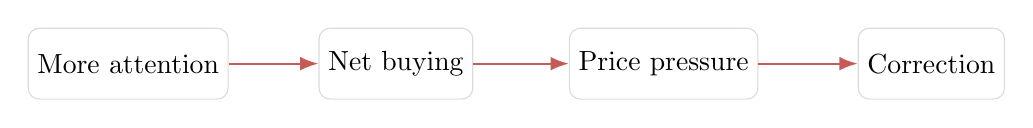
\begin{tikzpicture}[>=Latex,every node/.style={rounded corners,draw=rule,fill=white,minimum height=.9cm,align=center}]
\node (a) at (0,0) {More attention};
\node (b) at (3.4,0) {Net buying};
\node (c) at (6.8,0) {Price pressure};
\node (d) at (10.2,0) {Correction};
\draw[->,thick,rose] (a)--(b);\draw[->,thick,rose] (b)--(c);\draw[->,thick,rose] (c)--(d);
\end{tikzpicture}
\end{center}
\gap
\pair{plainbox}{On the attention day}{Buying can push prices above fundamentals.}
     {rosebox}{Over the next week}{As pressure fades, subsequent returns may turn negative.}
\end{frame}

% 07
\begin{frame}[t]{Retail channel III: when should reversal be stronger?}
\K{Price pressure persists when arbitrage is difficult}
\tri{rosebox}{High VIX}{Liquidity providers demand more compensation for risk.}
    {rosebox}{Wide spreads}{A given order imbalance creates more price impact.}
    {rosebox}{High lending fees}{Short-sale trades that correct prices cost more.}
\gap
\begin{center}\large\red{Prediction:} ARA has a more negative future-return coefficient in these states.\end{center}
\end{frame}

% 08
\begin{frame}[t]{Institutional channel: why attention rises before news}
\K{Research capacity can be allocated ahead of an event}
\begin{center}
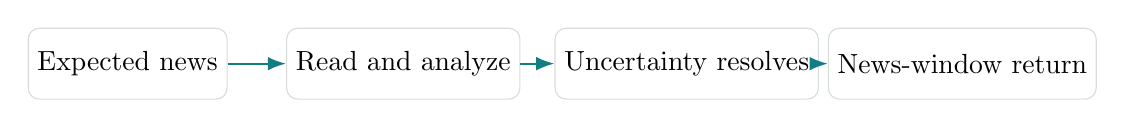
\begin{tikzpicture}[>=Latex,every node/.style={rounded corners,draw=rule,fill=white,minimum height=.9cm,align=center}]
\node (a) at (0,0) {Expected news};
\node (b) at (3.5,0) {Read and analyze};
\node (c) at (7.1,0) {Uncertainty resolves};
\node (d) at (10.6,0) {News-window return};
\draw[->,thick,teal] (a)--(b);\draw[->,thick,teal] (b)--(c);\draw[->,thick,teal] (c)--(d);
\end{tikzpicture}
\end{center}
\gap
\pair{tealbox}{Key condition}{Ahead of major news, attention may signal that an event matters to many stocks.}
     {plainbox}{Full sample}{Without an event condition, the positive association can be diluted.}
\take{The conditional premium can reflect risk-premium realization or resolution of uncertainty.}
\end{frame}

% 09
\begin{frame}[t]{Two attention measures, two testable predictions}
\K{Different mechanisms require different tests}
\numtable{\begin{tabularx}{\linewidth}{p{3.1cm}XX}\toprule
 & \red{Retail ARA} & \blue{Institutional AIA}\\\midrule
Baseline & Lower return over the following week & Weak unconditional relation\\
Conditional effect & More negative when market frictions rise & More positive before major news\\
Interpretation & Buying pressure followed by correction & Information processing and uncertainty resolution\\\bottomrule
\end{tabularx}}
\gap
\begin{beamercolorbox}[wd=\linewidth,sep=9pt,rounded=true]{plainbox}
The core tables ask, in order: \textbf{Does it predict? When is it stronger? What mechanism fits?}
\end{beamercolorbox}
\end{frame}

% 10
\begin{frame}[t]{Sample and data: from stocks to the market}
\K{The published study's common framework}
\pair{plainbox}{Stock universe}{US common shares on NYSE, AMEX, NASDAQ, and NYSE Arca, aligned with firm market value.}
     {plainbox}{Coverage}{ARA: July 2004--December 2019.\par AIA: available from February 2010.}
\gap
\tri{rosebox}{Retail input}{Google search volume}
    {tealbox}{Institutional input}{Bloomberg readership}
    {goldbox}{Market return}{CRSP value-weighted index}
\end{frame}

\begin{frame}[t]{Sample construction matters for the market test}
\K{The paper does not use a current index membership list}
\pair{plainbox}{Eligibility}{CRSP common-share codes 10 and 11; stocks closing below \$5 are excluded.}
     {plainbox}{Coverage shift}{Google attention begins in 2004; Bloomberg readership begins in 2010.}
\gap
\begin{beamercolorbox}[wd=\linewidth,sep=10pt,rounded=true]{goldbox}
Different ARA and AIA samples affect precision and complicate direct coefficient comparisons.
\end{beamercolorbox}
\end{frame}

% 11
\begin{frame}[t]{ARA begins with abnormal firm-level search}
\K{Google Search Volume Index / ASVI}
\begin{beamercolorbox}[wd=\linewidth,sep=13pt,rounded=true]{rosebox}
\centering\Large
$ASVI_{i,t}=\dfrac{SVI_{i,t}}{\operatorname{median}(SVI_{i,t-1:t-6m})}-1$
\end{beamercolorbox}
\gap
\pair{plainbox}{Why abnormal?}{Compare a stock with its own six-month history, rather than with other stocks' raw search volumes.}
     {plainbox}{What is observed?}{Active searches for a stock's name or ticker, rather than news volume or trading.}
\end{frame}

% 12
\begin{frame}[t]{Three details in constructing Google attention}
\K{Measurement choices affect the interpretation}
\tri{plainbox}{Ticker ambiguity}{Generic tickers are manually screened.}
    {plainbox}{Rolling baseline}{The benchmark must use information available before day $t$.}
    {plainbox}{Data vintages}{Daily SVI is a 0--100 relative score; vintages are cross-checked.}
\gap
\begin{beamercolorbox}[wd=\linewidth,sep=10pt,rounded=true]{rosebox}
These choices determine whether aggregated searches reliably represent retail attention.
\end{beamercolorbox}
\end{frame}

% 13
\begin{frame}[t]{AIA measures attention through Bloomberg readership}
\K{Turn firm-level reading intensity into a high-attention indicator}
\begin{beamercolorbox}[wd=\linewidth,sep=13pt,rounded=true]{tealbox}
\centering\Large
$HighInstAttention_{i,t}=\mathbb{1}(DMR_{i,t}\geq 3)$
\end{beamercolorbox}
\gap
\pair{plainbox}{DMR}{Maximum hourly Bloomberg readership, relative to the stock's prior 30 days.}
     {plainbox}{High attention}{Scores 3 or 4 exceed roughly the 94th percentile of past activity.}
\end{frame}

% 14
\begin{frame}[t]{From firms to the market: one aggregation rule}
\K{Larger firms receive greater weight}
\begin{beamercolorbox}[wd=\linewidth,sep=12pt,rounded=true]{plainbox}
\centering\Large
$ARA_t=\sum_i w_{i,t}ASVI_{i,t}
\qquad
AIA_t=\sum_i w_{i,t}HighInstAttention_{i,t}$
\end{beamercolorbox}
\gap
\pair{rosebox}{How to read ARA}{Market-wide abnormal search intensity.}
     {tealbox}{How to read AIA}{The value-weighted share of stocks receiving high institutional attention.}
\end{frame}

% 15
\begin{frame}[t]{Timing: attention first, returns later}
\K{The main outcome is the cumulative return on trading days $t+2$ through $t+6$}
\begin{center}
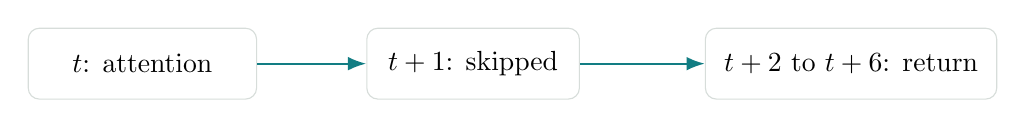
\begin{tikzpicture}[>=Latex]
\node[draw=rule,fill=white,rounded corners,minimum width=2.9cm,minimum height=.9cm] (a) at (0,0) {$t$: attention};
\node[draw=rule,fill=white,rounded corners,minimum width=2.7cm,minimum height=.9cm] (b) at (4.2,0) {$t+1$: skipped};
\node[draw=rule,fill=white,rounded corners,minimum width=3.7cm,minimum height=.9cm] (c) at (9.0,0) {$t+2$ to $t+6$: return};
\draw[->,thick,teal] (a)--(b);\draw[->,thick,teal] (b)--(c);
\end{tikzpicture}
\end{center}
\gap
\pair{plainbox}{Why skip a day?}{Calendar-day attention overlaps part of the next close-to-close return.}
     {plainbox}{Why a five-day window?}{To capture a short correction or returns around information release.}
\end{frame}

\begin{frame}[t]{The clock mismatch explains the skipped day}
\K{The timing choice follows how the source data define a day}
\pair{rosebox}{Google ARA}{The midnight-to-midnight GMT search window overlaps about four hours of the $t+1$ market return.}
     {tealbox}{Bloomberg AIA}{Calendar-day readership overlaps about eight hours of the $t+1$ return.}
\gap
\begin{beamercolorbox}[wd=\linewidth,sep=10pt,rounded=true]{plainbox}
Using $R_{t+2:t+6}$ keeps these overlapping hours out of the headline predictive test.
\end{beamercolorbox}
\end{frame}

% 16
\begin{frame}[t]{Regression: what else is controlled?}
\K{Predict future market returns with today's attention}
\begin{beamercolorbox}[wd=\linewidth,sep=11pt,rounded=true]{plainbox}
\centering\Large
$R_{t+2:t+6}=\alpha+\beta Attention_t+\gamma X_t+\varepsilon_t$
\end{beamercolorbox}
\gap
\tri{plainbox}{Macro and sentiment}{BW, TMS, DFY, $\Delta ADS$, $\Delta EPU$}
    {plainbox}{News and trading}{Abnormal news volume and turnover}
    {plainbox}{Market dynamics}{VIX, turnover, returns, and up to four lags}
\end{frame}

% 17
\begin{frame}[t]{Table 1: the two attention measures differ}
\K{Descriptive statistics in the published study}
\numtable{\begin{tabularx}{\linewidth}{p{3.7cm}cccX}\toprule
Measure & Trading days & Mean & Std. dev. & Persistence $\rho$\\\midrule
\red{ARA} & 3,903 & 0.065 & 0.054 & 0.77\\
\blue{AIA} & 2,431 & 0.254 & 0.100 & 0.57\\\bottomrule
\end{tabularx}}
\gap
\pair{plainbox}{Common component}{ARA and AIA have a correlation of about 0.282; they are not independent.}
     {plainbox}{Important differences}{Their volatility, persistence, and economic meanings are distinct.}
\end{frame}

\begin{frame}[t]{Aggregation reveals a persistent common component}
\K{Market attention outlasts the average firm-specific shock}
\numtable{\begin{tabularx}{\linewidth}{p{4.4cm}XX}\toprule
Autocorrelation & Aggregate measure & Average firm-level measure\\\midrule
Retail attention & $0.77$ & $0.41$\\
Institutional attention & $0.57$ & $0.24$\\\bottomrule
\end{tabularx}}
\gap
\pair{plainbox}{Reading}{Shared shocks persist after firm-specific noise is averaged out.}
     {plainbox}{Caution}{Attention is still less persistent than VIX and yield spreads.}
\end{frame}

% 18
\begin{frame}[t]{Dynamics: which attention measure tends to lead?}
\K{The paper studies lead--lag relations with a VAR}
\pair{tealbox}{After an AIA shock}{ARA's cumulative response reaches about $0.219$ by day nine and remains significant.}
     {rosebox}{After an ARA shock}{AIA's initial response is about $0.079$ and is not significant.}
\gap
\begin{center}\large\blue{Institutional attention} $\longrightarrow$ \red{Retail attention}\end{center}
\take{Impulse responses describe dynamic association; they do not establish causation.}
\end{frame}

% 19
\begin{frame}[t]{Table 2: establish the baseline first}
\K{The same return windows are tested with ARA and AIA separately}
\pair{rosebox}{Panel A: ARA}{Track each day from $t+1$ to $t+6$, then the cumulative return from $t+2$ to $t+6$.}
     {tealbox}{Panel B: AIA}{Use the same timing; add ARA in one specification to distinguish the two signals.}
\gap
\begin{beamercolorbox}[wd=\linewidth,sep=10pt,rounded=true]{plainbox}
\centering \large Establish the \textbf{average predictive relation} before conditioning on states and events.
\end{beamercolorbox}
\end{frame}

% 20
\begin{frame}[t]{Table 2A: ARA predicts subsequent daily returns}
\K{Published results / retail attention}
\numtable{\begin{tabularx}{\linewidth}{p{3.2cm}cccX}\toprule
Return day & $t+1$ & $t+2$ & $t+6$ & Pattern\\\midrule
ARA coefficient & $-0.814^{**}$ & $-0.902^{**}$ & $-0.805^{***}$ & Negative on several future days\\
NW $t$ & $-2.24$ & $-2.30$ & $-2.64$ & Persists beyond day one\\\bottomrule
\end{tabularx}}
\gap
\pair{rosebox}{Direction}{Higher ARA is followed by lower daily market returns.}
     {plainbox}{Timing}{The main test starts at $t+2$ to reduce ambiguity around measurement and nearby returns.}
\end{frame}

% 21
\begin{frame}[t]{Table 2A: the economic magnitude over one week}
\K{Published result / controlled $t+2:t+6$ specification}
\begin{center}
{\fontsize{31}{36}\selectfont\red{$\beta=-4.137^{***}$}}\par
\vspace{.12cm}
{\large Newey--West $t=-2.86$}
\end{center}
\gap
\pair{plainbox}{One typical change}{A one-standard-deviation rise in ARA corresponds to about 22.34 bp lower market return over the following week.}
     {rosebox}{Mechanism link}{Consistent with retail buying pressure followed by a correction.}
\end{frame}

% 22
\begin{frame}[t]{Table 2B: AIA's daily signal is different}
\K{Published results / institutional attention}
\numtable{\begin{tabularx}{\linewidth}{p{3.0cm}cccX}\toprule
Return day & $t+1$ & $t+2$ & $t+6$ & Interpretation\\\midrule
AIA coefficient & $0.396^{*}$ & $0.240$ & $0.053$ & Most daily results are not significant\\
NW $t$ & $1.75$ & $1.18$ & $0.32$ & Unlike ARA's timing pattern\\\bottomrule
\end{tabularx}}
\gap
\begin{beamercolorbox}[wd=\linewidth,sep=10pt,rounded=true]{tealbox}
The positive signal from institutional attention may require a \textbf{major information event}, rather than an arbitrary trading day.
\end{beamercolorbox}
\end{frame}

% 23
\begin{frame}[t]{Table 2B: weak full-sample weekly predictability}
\K{Published result / controlled $t+2:t+6$ specification}
\pair{tealbox}{AIA alone}{Coefficient $0.927$; NW $t=1.52$, below conventional significance thresholds.}
     {plainbox}{Controlling for ARA}{AIA coefficient $1.089^{*}$; NW $t=1.72$, still relatively weak evidence.}
\gap
\begin{center}\Large\blue{Next question:} Is AIA informative specifically before announcements?\end{center}
\end{frame}

% 24
\begin{frame}[t]{Partial replication: retained and substituted inputs}
\K{The feasible specification for Tables 2--4}
\numtable{\begin{tabularx}{\linewidth}{p{3.6cm}YY}\toprule
Element & Published study & Replication exercise\\\midrule
Retail attention & Google ARA & Authors' released ARA\\
Institutional attention & Bloomberg AIA & Abnormal index-options volume proxy\\
Market return & CRSP broad market & S\&P 500 proxy\\
Sample & Separate ARA and AIA coverage & 2010--19; 2,437 common trading days\\
Abnormal news volume & Included control & Unavailable; omitted\\\bottomrule
\end{tabularx}}
\end{frame}

% 25
\begin{frame}[t]{Table 2 replication: ARA retains the negative sign}
\K{Controlled return over the following week}
\numtable{\begin{tabularx}{\linewidth}{p{4.0cm}XX}\toprule
 & Published study & Replication\\\midrule
Coefficient & $-4.137^{***}$ & $-1.363$\\
NW30 $t$ & $-2.86$ & $-1.10$\\
One-SD effect & $-22.34$ bp & $-7.28$ bp\\
Trading days & 3,903 & 2,437\\\bottomrule
\end{tabularx}}
\gap
\begin{beamercolorbox}[wd=\linewidth,sep=10pt,rounded=true]{rosebox}
\textbf{Reading:} The sign matches, but the estimated effect is smaller and statistically inconclusive in the replication.
\end{beamercolorbox}
\end{frame}

% 26
\begin{frame}[t]{Table 2 replication: the AIA proxy is insignificant}
\K{Controlled return over the following week}
\numtable{\begin{tabularx}{\linewidth}{p{4.0cm}XX}\toprule
 & Original Bloomberg AIA & Options-volume proxy\\\midrule
Coefficient & $0.927$ & $0.197$\\
NW30 $t$ & $1.52$ & $1.10$\\
Trading days & 2,431 & 2,437\\\bottomrule
\end{tabularx}}
\gap
\pair{tealbox}{Similarity}{Neither weekly full-sample estimate provides strong evidence.}
     {plainbox}{Boundary}{Readership and options trading are different measures; coefficient sizes are not directly comparable.}
\end{frame}

% 27
\begin{frame}[t]{Table 2 in one slide: a baseline and a condition}
\K{The next tests examine mechanisms}
\pair{rosebox}{ARA}{Significantly negative in the paper; negative but insignificant in the replication. Next: do market frictions amplify it?}
     {tealbox}{AIA}{Limited full-sample evidence. Next: does the signal appear before announcements?}
\gap
\begin{center}\large
\red{Table 3: market states} \qquad \blue{Table 4: news events}
\end{center}
\end{frame}

% 28
\begin{frame}[t]{Table 3: bring market frictions into the test}
\K{If price pressure is the channel, market states should change its strength}
\tri{plainbox}{High VIX}{Liquidity providers are more sensitive to risk.}
    {plainbox}{Wide effective spreads}{Trading pressure is harder to absorb.}
    {plainbox}{High stock-lending fees}{Short-sale correction becomes more costly.}
\gap
\begin{beamercolorbox}[wd=\linewidth,sep=10pt,rounded=true]{rosebox}
Split the sample by state, compare ARA coefficients, and test the high-minus-low difference.
\end{beamercolorbox}
\end{frame}

% 29
\begin{frame}[t]{Table 3: stronger reversal when VIX is high}
\K{Published result / VIX split}
\numtable{\begin{tabularx}{\linewidth}{p{3.8cm}cccX}\toprule
ARA & High VIX & Low VIX & High minus low & Interpretation\\\midrule
Coefficient & $-5.167$ & $-1.170$ & $-3.997$ & Negative difference\\
White $t$ & $-2.92^{***}$ & $-1.23$ & $-1.99^{**}$ & Stronger in high VIX\\
One-SD effect & $-27.96$ bp & $-6.29$ bp & &\\\bottomrule
\end{tabularx}}
\gap
\take{In the published results, retail attention predicts a larger reversal during high-volatility states.}
\end{frame}

% 30
\begin{frame}[t]{Table 3: two other frictions point in the same direction}
\K{Published results / these splits are outside the replication}
\pair{rosebox}{Effective spreads}{ARA coefficient: $-6.303$ in the high-spread group versus $-0.667$ in the low-spread group.}
     {rosebox}{Stock-lending fees}{ARA coefficient: $-17.968$ in the high-fee group versus $-4.000$ in the low-fee group.}
\gap
\begin{beamercolorbox}[wd=\linewidth,sep=10pt,rounded=true]{plainbox}
All three splits fit the idea that stronger frictions slow correction of short-lived buying pressure.
\end{beamercolorbox}
\end{frame}

% 31
\begin{frame}[t]{Table 3 replication: ARA's VIX difference is uncertain}
\K{Only the VIX split was reconstructed / replication uses NW30 inference}
\numtable{\begin{tabularx}{\linewidth}{p{3.8cm}cccX}\toprule
ARA & High VIX & Low VIX & High minus low & NW30 $t$\\\midrule
Replication coefficient & $-2.192$ & $-0.692$ & $-1.500$ & $-1.11,\ -0.29,\ -0.43$\\
Published coefficient & $-5.167$ & $-1.170$ & $-3.997$ & Paper also reports White $t$\\\bottomrule
\end{tabularx}}
\gap
\pair{rosebox}{Point estimates}{The high-VIX coefficient is more negative, as in the paper.}
     {plainbox}{Inference}{The high-minus-low difference is not significant in the replication.}
\end{frame}

% 32
\begin{frame}[t]{Table 3 replication: the AIA proxy across VIX states}
\K{The inference method matters}
\numtable{\begin{tabularx}{\linewidth}{p{3.8cm}cccX}\toprule
AIA & High VIX & Low VIX & High minus low & Difference $t$\\\midrule
Published study & $1.480$ & $-0.200$ & $1.680$ & White $1.96^{**}$\\
Options-volume proxy & $0.326$ & $-0.166$ & $0.491$ & White $1.81^{*}$\\
Replication NW30 & & & & $1.43$\\\bottomrule
\end{tabularx}}
\gap
\take{The proxy offers weak 10\% evidence with White errors, but not after allowing for time dependence.}
\end{frame}

% 33
\begin{frame}[t]{Table 3 synthesis: separate direction from mechanism}
\K{How to read the state tests}
\pair{rosebox}{Published pattern}{ARA is more negative under high VIX, wide spreads, and high lending fees.}
     {tealbox}{Replication pattern}{The high-VIX point estimate is more negative, but the difference is not robustly significant.}
\gap
\begin{beamercolorbox}[wd=\linewidth,sep=10pt,rounded=true]{plainbox}
An additional TED-spread analysis concerns \textbf{funding stress}; it is not a measure of stock-lending fees and cannot replace that test.
\end{beamercolorbox}
\end{frame}

% 34
\begin{frame}[t]{Table 4: attention before news}
\K{A weak full-sample effect can hide a conditional relation}
\begin{center}

\begin{tikzpicture}[>=Latex]
\node[draw=rule,fill=white,rounded corners,minimum width=3.0cm,minimum height=.9cm] (a) at (0,0) {Attention before news};
\node[draw=rule,fill=white,rounded corners,minimum width=3.0cm,minimum height=.9cm] (b) at (4.2,0) {Major announcement};
\node[draw=rule,fill=white,rounded corners,minimum width=3.3cm,minimum height=.9cm] (c) at (8.8,0) {Uncertainty resolves};
\draw[->,thick,teal] (a)--(b);\draw[->,thick,teal] (b)--(c);
\end{tikzpicture}
\end{center}
\gap
\pair{tealbox}{Prediction}{AIA's positive coefficient is larger if a major announcement occurs in the future-return window.}
     {plainbox}{Comparison}{Days when that future window has no announcement.}
\end{frame}

\begin{frame}[t]{Two explanations for the AIA news-window premium}
\K{The paper treats these channels as compatible, not mutually exclusive}
\pair{tealbox}{Risk-premium timing}{Announcements carrying systematic information can concentrate expected equity premia near release.}
     {plainbox}{Uncertainty resolution}{High institutional attention can signal elevated, anticipated market uncertainty before news.}
\gap
\begin{beamercolorbox}[wd=\linewidth,sep=10pt,rounded=true]{goldbox}
Table 4 shows a conditional predictive association; it does not by itself identify which channel dominates.
\end{beamercolorbox}
\end{frame}

% 35
\begin{frame}[t]{Table 4: what counts as a news window?}
\K{The announcement must occur between $t+2$ and $t+6$}
\pair{tealbox}{Macro News}{FOMC meetings, nonfarm payrolls, or PPI releases.}
     {plainbox}{All News}{Macro news or days in the top 5\% of announcing firms' market-capitalization share.}
\gap
\begin{beamercolorbox}[wd=\linewidth,sep=10pt,rounded=true]{goldbox}
The split is based on \textbf{whether an announcement occurs}, not whether its content is good or bad.
\end{beamercolorbox}
\end{frame}

\begin{frame}[t]{Institutional attention rises before scheduled news}
\K{The event split is also reflected in the attention series itself}
\numtable{\begin{tabularx}{\linewidth}{p{5.2cm}XX}\toprule
Mean AIA & Before major news & Other days\\\midrule
Published sample & $0.266$ & $0.241$\\\bottomrule
\end{tabularx}}
\gap
\pair{tealbox}{Evidence}{The difference is statistically strong ($t=5.84$).}
     {plainbox}{Interpretation}{Institutions allocate more attention before events that can affect many firms.}
\end{frame}

% 36
\begin{frame}[t]{Table 4A: AIA's positive signal appears around news}
\K{Published result / Macro News}
\numtable{\begin{tabularx}{\linewidth}{p{3.8cm}cccX}\toprule
AIA & News & No news & News minus no news & White $t$: news; diff.\\\midrule
Coefficient & $2.076$ & $-0.375$ & $2.451$ & $3.20^{***};\ 2.78^{***}$\\
One-SD effect & $+20.82$ bp & $-3.74$ bp & &\\\bottomrule
\end{tabularx}}
\gap
\pair{tealbox}{Key comparison}{The news-window coefficient is positive, and the between-window difference is significant.}
     {plainbox}{Mechanism link}{Institutional attention may reflect deliberate analysis before news resolves uncertainty.}
\end{frame}

\begin{frame}[t]{Does AIA simply capture informed front-running?}
\K{The paper checks returns before scheduled macro announcements}
\pair{plainbox}{Pre-event window}{Correlations between AIA and market returns from $t-4$ to $t$ are small: $0.011$ to $0.038$.}
     {tealbox}{Interpretation}{No notable pre-release return pattern appears; this is consistent with uncertainty being anticipated.}
\gap
\begin{beamercolorbox}[wd=\linewidth,sep=10pt,rounded=true]{goldbox}
The check narrows one alternative explanation, but it is not a complete test of private information trading.
\end{beamercolorbox}
\end{frame}

% 37
\begin{frame}[t]{Table 4B: ARA's news-window difference}
\K{Published result / Macro News}
\numtable{\begin{tabularx}{\linewidth}{p{3.8cm}cccX}\toprule
ARA & News & No news & News minus no news & White $t$\\\midrule
Coefficient & $-2.505$ & $-5.225$ & $2.720$ & $-1.69^{*},\ -4.50^{***},\ 1.44$\\\bottomrule
\end{tabularx}}
\gap
\pair{rosebox}{Different from AIA}{ARA remains mainly negative; its between-window difference is insignificant.}
     {plainbox}{Interpretation}{Retail pressure and institutional pre-news analysis imply different return paths.}
\end{frame}

% 38
\begin{frame}[t]{How was the Macro News indicator reconstructed?}
\K{Preserve the event definition while recognizing differences in implementation}
\tri{plainbox}{Real dates}{Use official FOMC, payroll, and PPI announcement calendars.}
    {plainbox}{Future window}{Mark whether an event falls on trading days $t+2$ through $t+6$.}
    {plainbox}{Regression sample}{1,324 news-window days and 1,113 non-news days.}
\gap
\begin{beamercolorbox}[wd=\linewidth,sep=10pt,rounded=true]{tealbox}
Event selection and holiday treatment may differ from the paper. AIA remains an options-volume proxy, and abnormal news volume is omitted as a control.
\end{beamercolorbox}
\end{frame}

% 39
\begin{frame}[t]{Table 4 replication: no significant AIA news effect}
\K{Macro News / index-options-volume proxy}
\numtable{\begin{tabularx}{\linewidth}{p{3.8cm}cccX}\toprule
 & News & No news & News minus no news & Difference $t$\\\midrule
Original AIA & $2.076$ & $-0.375$ & $2.451$ & White $2.78^{***}$\\
Options-volume proxy & $0.280$ & $0.209$ & $0.071$ & NW30 $0.22$\\\bottomrule
\end{tabularx}}
\gap
\pair{tealbox}{Point estimate}{The coefficient on news-window days is positive.}
     {plainbox}{Decisive contrast}{The difference from non-news days is near zero and insignificant.}
\end{frame}

% 40
\begin{frame}[t]{Replication: ARA's news-window difference}
\K{Macro News / retail attention}
\numtable{\begin{tabularx}{\linewidth}{p{3.8cm}cccX}\toprule
 & News & No news & News minus no news & Difference $t$\\\midrule
Published study & $-2.505$ & $-5.225$ & $2.720$ & White $1.44$\\
Replication & $-2.333$ & $0.322$ & $-2.655$ & NW30 $-1.17$\\\bottomrule
\end{tabularx}}
\gap
\pair{rosebox}{Common feature}{Neither between-window difference is significant.}
     {plainbox}{Important difference}{Their signs differ, so the results are not uniformly aligned.}
\end{frame}

% 41
\begin{frame}[t]{Table 4 synthesis: the window difference is central}
\K{Do not read one positive coefficient in isolation}
\pair{tealbox}{Published claim}{AIA's positive predictability rises significantly before major announcements.}
     {plainbox}{Replication evidence}{The proxy's news-minus-no-news difference is insignificant.}
\gap
\begin{beamercolorbox}[wd=\linewidth,sep=10pt,rounded=true]{goldbox}
The replication does not refute the original AIA result: it observes options trading, while the paper observes Bloomberg readership.
\end{beamercolorbox}
\end{frame}

% 42
\begin{frame}[t]{Section 2.4: does retail attention accompany buying?}
\K{Published trading evidence}
\pair{rosebox}{Retail order imbalance}{ARA is positively associated with measures of net retail buying.}
     {rosebox}{Mutual-fund flows}{ARA is also positively associated with equity-fund inflows.}
\gap
\numtable{\begin{tabularx}{\linewidth}{p{5.1cm}XX}\toprule
Contemporaneous trading outcome & Coefficient & NW $t$\\\midrule
ARA $\rightarrow$ ROIB1 & $3.555^{**}$ & $2.25$\\
ARA $\rightarrow$ fund flow & $0.187^{**}$ & $2.42$\\\bottomrule
\end{tabularx}}
\end{frame}

% 43
\begin{frame}[t]{Section 2.4: retail buying on down-market days}
\K{Published trading evidence}
\pair{rosebox}{Negative-return days}{The association between ARA and net retail buying is stronger, consistent with contrarian purchases.}
     {plainbox}{Extreme down days}{The buying measures remain positive when market returns are in the bottom 5\% of the sample.}
\gap
\begin{beamercolorbox}[wd=\linewidth,sep=10pt,rounded=true]{goldbox}
Buying even after bad news can create short-lived support for prices followed by a correction.
\end{beamercolorbox}
\end{frame}

\begin{frame}[t]{Out-of-sample forecast design}
\K{The paper moves from fitted relationships to implementable predictions}
\tri{plainbox}{Rolling estimation}{Estimate a univariate attention regression on a 500-day window.}
    {plainbox}{Benchmark}{Use the historical mean return from the same window.}
    {plainbox}{Evaluation}{Compare forecast errors for the $t+2:t+6$ return.}
\gap
\pair{rosebox}{ARA test starts}{August 2006, after the initial training period.}
     {tealbox}{AIA test starts}{March 2012, after Bloomberg coverage allows training.}
\end{frame}

% 44
\begin{frame}[t]{Section 2.5: does predictability survive out of sample?}
\K{Published Table 5}
\numtable{\begin{tabularx}{\linewidth}{p{3.5cm}cccX}\toprule
Out-of-sample $R^2$ & Full sample & Relevant state & Comparison & Pattern\\\midrule
ARA & $1.49\%^{**}$ & High VIX $2.70\%^{***}$ & Low VIX $-0.39\%$ & State dependence\\
AIA & $-0.36\%$ & Macro News $1.19\%^{*}$ & No news $-0.39\%$ & Event dependence\\\bottomrule
\end{tabularx}}
\gap
\take{The out-of-sample pattern mirrors the paper's central distinction: frictions for retail, news for institutions.}
\end{frame}

\begin{frame}[t]{Does forecasting improve allocation?}
\K{The paper adds an economic, rather than only statistical, test}
\pair{plainbox}{Portfolio rule}{A mean--variance investor splits wealth between the market and Treasury bills using the return forecast.}
     {plainbox}{Assumptions}{Risk aversion is 3; the reported strategy includes 50 bp transaction costs.}
\gap
\numtable{\begin{tabularx}{\linewidth}{p{4.5cm}XX}\toprule
Annual certainty-equivalent gain & Full sample & Strongest relevant state\\\midrule
ARA & $2.26\%$ & High VIX $2.76\%$\\
AIA & $-0.74\%$ & Macro News $1.83\%$\\\bottomrule
\end{tabularx}}
\end{frame}

% 45
\begin{frame}[t]{Section 2.6: are the results robust to other choices?}
\K{Published Table 6}
\tri{plainbox}{Time and sample}{Exclude the crisis or December; add weekday effects.}
    {plainbox}{Inference}{Change standard errors, add lagged attention, or smooth attention.}
    {plainbox}{Measures}{Use S\&P 500 returns or alternative value weights.}
\gap
\pair{rosebox}{ARA}{The coefficient remains negative in most checks.}
     {tealbox}{AIA around news}{The conditional coefficient remains positive in most checks.}
\end{frame}

\begin{frame}[t]{Alternative aggregation: what if mega-caps dominate?}
\K{Published Table 6, Panel B}
\pair{plainbox}{Reweighting}{Use capped market-value weights, equal weights, principal components, or partial least squares.}
     {tealbox}{Result}{PLS attention is stronger: ARA has OOS $R^2=2.14\%$; AIA in All News windows has $R^2=1.36\%$.}
\gap
\begin{beamercolorbox}[wd=\linewidth,sep=10pt,rounded=true]{goldbox}
The main effects survive substantial reductions in mega-cap weight; they are not driven by a few giant firms.
\end{beamercolorbox}
\end{frame}

\begin{frame}[t]{Why bottom-up attention beats top-down proxies}
\K{Published Table 6, Panel C}
\pair{rosebox}{Retail}{Searches for market-index terms do not predict returns reliably out of sample. Retail investors often hold and trade individual stocks.}
     {tealbox}{Institutional}{Readership of SPY alone is weaker than the share of individual stocks receiving high Bloomberg attention.}
\gap
\begin{beamercolorbox}[wd=\linewidth,sep=10pt,rounded=true]{plainbox}
Bottom-up AIA also signals how broadly an upcoming event matters across the stock universe.
\end{beamercolorbox}
\end{frame}

\begin{frame}[t]{Cross-sectional design: test exposure to each channel}
\K{Published Table 7 asks where market-level predictability should be strongest}
\pair{rosebox}{Liquidity portfolios}{Sort stocks by past-month Amihud illiquidity; compare the most liquid and least liquid quintiles.}
     {tealbox}{Beta portfolios}{Estimate CAPM beta from rolling monthly returns; compare low- and high-beta quintiles around news.}
\gap
\begin{beamercolorbox}[wd=\linewidth,sep=10pt,rounded=true]{goldbox}
These sorts test price-impact sensitivity for ARA and systematic-risk exposure for AIA.
\end{beamercolorbox}
\end{frame}

% 46
\begin{frame}[t]{Section 2.7: which portfolios bear more of the effect?}
\K{Published Table 7}
\pair{rosebox}{Liquidity sorting}{ARA's negative predictability is stronger for illiquid stocks.\par Full sample: $-3.443$ for the most liquid portfolio versus $-5.675$ for the least liquid.}
     {tealbox}{Beta sorting}{Before major news, AIA's positive predictability is stronger for high-beta stocks.\par Macro News: $1.284$ for low beta versus $3.512$ for high beta.}
\gap
\begin{beamercolorbox}[wd=\linewidth,sep=10pt,rounded=true]{plainbox}
The cross-section connects the two channels to \textbf{liquidity exposure} and \textbf{market-risk exposure}.
\end{beamercolorbox}
\end{frame}

\begin{frame}[t]{Distraction instrument: what variation is used?}
\K{The paper seeks attention shocks unrelated to stock fundamentals}
\pair{rosebox}{Construct Dist}{Take the top 10\% of news-pressure days within each year, based on sensational broadcast-news coverage.}
     {plainbox}{Restrict the sample}{Exclude scheduled macro news, extreme market moves, and the crisis period to limit direct market-news channels.}
\gap
\begin{beamercolorbox}[wd=\linewidth,sep=10pt,rounded=true]{goldbox}
The identifying assumption is that these distractions affect future returns through retail attention rather than another channel.
\end{beamercolorbox}
\end{frame}

% 47
\begin{frame}[t]{Section 3.1: news distraction as an attention shock}
\K{Published Table 8}
\pair{rosebox}{First stage}{On high-news-pressure distraction days, ARA falls: coefficient $-0.014^{***}$ and first-stage $F=19.673$.}
     {plainbox}{Second stage}{Instrumented ARA predicts future returns with coefficient $-23.737$; NW $t=-1.87^{*}$.}
\gap
\begin{beamercolorbox}[wd=\linewidth,sep=10pt,rounded=true]{goldbox}
The instrument is weak for AIA ($F=0.687$), so it offers no strong causal evidence for the institutional channel.
\end{beamercolorbox}
\end{frame}

\begin{frame}[t]{The clustered-earnings puzzle comes before the release}
\K{Why is an after-hours announcement associated with an earlier market premium?}
\pair{plainbox}{Event definition}{In January, April, July, and October, identify the four days with the greatest announcing-firm market capitalization.}
     {rosebox}{Timing puzzle}{For clustered after-hours releases, the market earns about 17.16 bp on the event day, before the news arrives.}
\gap
\begin{beamercolorbox}[wd=\linewidth,sep=10pt,rounded=true]{tealbox}
Split these days by ARA: if retail buying pressure matters, the early premium should be concentrated on high-ARA days.
\end{beamercolorbox}
\end{frame}

% 48
\begin{frame}[t]{Section 3.2: clustered earnings and return timing}
\K{Published Figure 3 and Table 9}
\pair{rosebox}{High-ARA after-hours earnings days}{The same-day coefficient is $+33.478$ bp and significant; the next-day coefficient is $-9.794$ bp and insignificant.}
     {plainbox}{Low-ARA after-hours earnings days}{The same-day coefficient is $+9.396$ bp and insignificant; the next-day coefficient is $+26.455$ bp and significant.}
\gap
\begin{beamercolorbox}[wd=\linewidth,sep=10pt,rounded=true]{tealbox}
Retail buying before an announcement can change which day captures the return premium.
\end{beamercolorbox}
\end{frame}

% 49
\begin{frame}[t]{Final synthesis: the paper and the replication}
\K{Return to the two paths}
\tri{rosebox}{Retail in the paper}{ARA $\rightarrow$ buying pressure $\rightarrow$ reversal; stronger under market frictions.}
    {tealbox}{Institutional in the paper}{AIA $\rightarrow$ pre-news analysis $\rightarrow$ positive news-window returns.}
    {goldbox}{Partial replication}{Some point-estimate signs align, but robust significance in Tables 2--4 is not recovered.}
\gap
\begin{beamercolorbox}[wd=\linewidth,sep=11pt,rounded=true]{plainbox}
\centering\large\bfseries
Who pays attention shapes the mechanism; when they pay attention determines when it appears in returns.
\end{beamercolorbox}
\end{frame}
\end{document}


